% !TEX program = pdflatex
% !TEX encoding = UTF-8
% !BIB program = biber
% !TEX spellcheck = en_US
\documentclass[13pt,aspectratio=169]{beamer}

\usetheme{Berkeley}
\usecolortheme{crane}
\makeatletter
\beamer@headheight=1.5\baselineskip
\makeatother
\setbeamertemplate{navigation symbols}{}
\addtobeamertemplate{navigation symbols}{}{%
	\usebeamerfont{footline}%
	\usebeamercolor[fg]{footline}%
	\hspace{1em}%
	\insertframenumber/\inserttotalframenumber
}
\setbeamertemplate{caption}[numbered]
\setbeamercovered{transparent}

\usepackage[utf8]{inputenc}
\usepackage{amsmath}
\usepackage{amsfonts}
\usepackage{amssymb}
\usepackage{graphicx}
\usepackage[version=4]{mhchem}
\usepackage{siunitx}
\usepackage[figurename=Fig.]{caption}
\usepackage{bm}
\usepackage[bibstyle=nature,backend=biber]{biblatex}

\newcommand*{\rmn}[1]{\romannumeral#1}
\newcommand*{\RMN}[1]{\uppercase\expandafter{\romannumeral#1}}
\DeclareCiteCommand{\footcite}[\mkbibfootnote]
	{\usebibmacro{prenote}}
	{\printnames[family-given]{labelname}%
		\newunit
		\printfield{journaltitle}%
		\newunit
		\printfield{year}
		\newunit
		\printlabeldateextra
	}
	{\addsemicolon\space}
	{\usebibmacro{postnote}
}
\DeclareCiteCommand{\footcitetext}[\footnotetext]
	{\usebibmacro{prenote}}
	{\printnames[family-given]{labelname}%
		\newunit
		\printfield{journaltitle}%
		\newunit
		\printfield{year}
	}
	{\addsemicolon\space}
	{\usebibmacro{postnote}
}

\author[Qi Zhang et. al.]{\underline{Qi Zhang} \inst{1} \and Tian Qin \inst{2} \and Renata Wentzcovitch\inst{1,3} \and Koichiro Umemoto\inst{4}}
\institute{\inst{1} Applied Physics and Applied Mathematics Department, Columbia University, New York, NY \and%
	\inst{2} Department of Earth Sciences, University of Minnesota, Minneapolis, MN \and%
\inst{3} Lamont-Doherty Earth Observatory, Columbia University, Palisades, NY \and%
\inst{4} Earth-Life Science Institute, Tokyo Institute of Technology}
\title[\texttt{qha}]{\texttt{qha}: A Python package for quasi-harmonic free energy calculation for multi-configuration systems\footcite{qin2018qha}}
\date{}

\addbibresource{ref.bib}

\begin{document}

\begin{frame}
	\titlepage
\end{frame}

\section{Introduction}

\subsection{Quasi-harmonic approximation (QHA)}
\begin{frame}{\subsecname}
	\begin{itemize}[<+(1)->]
		\setlength\itemsep{1em}
		\item a useful tool to compute materials thermodynamic properties at high $T$, $P$
		\item a good approximation up to about $0.7 T_\text{melting}$
		\item static contribution by (DFT, AIMD), vibrational contribution: DFPT followed by QHA
		\item deal with multiple configuration systems
	\end{itemize}
\end{frame}

\subsection{Multi-configuration system that \texttt{qha} may apply}
\begin{frame}{\subsecname}
	\begin{itemize}[<+(1)->]
		\setlength\itemsep{1em}
		\item the order-disorder phase boundary between ice-\RMN{8} and ice-\RMN{7} \footcite{umemoto2010order},
		\item the relative stability of hydrous defects in \ce{Mg2SiO4}-forsterite at high $P$ and $T$ \footcite{qin2018ab},
		\item the effect of disorder and iron concentration on the spin crossover diagram of \ce{Fe^3+}-bearing \ce{MgSiO3}-bridgmanite \footcite{shukla2016spin}.
	\end{itemize}
\end{frame}

\subsection{Methods}
\begin{frame}{\subsecname}
	\begin{itemize}[<+(1)->]
		\item single configuration system:
		      \begin{align}
			      Z(T, v) & = \exp\big( -{E(v)}/{k_B T} \big) \prod_{\bm{q}, s} \frac{\exp(-\hbar \omega_{\bm{q}s}(v)/2k_B T)}{1 - \exp(-\hbar \omega_{\bm{q}s}(v)/k_B T)}, \\
			      F(T, v) & = -k_B T \ln Z(T, v),
		      \end{align}
		\item multi-configuration systems:
		      \begin{align}
			      Z(T, v) & = \sum_{n=1}^{N_c} g_n Z_n (T, v), \\
			      F(T, v) & = -k_B T \ln Z(T, v).
		      \end{align}
		\item finite strain equation of state fitting to string $\{F(T, v)\}$’s to a continuous function $F(T, V)$
	\end{itemize}
\end{frame}

\begin{frame}{\subsecname}
	\centering
	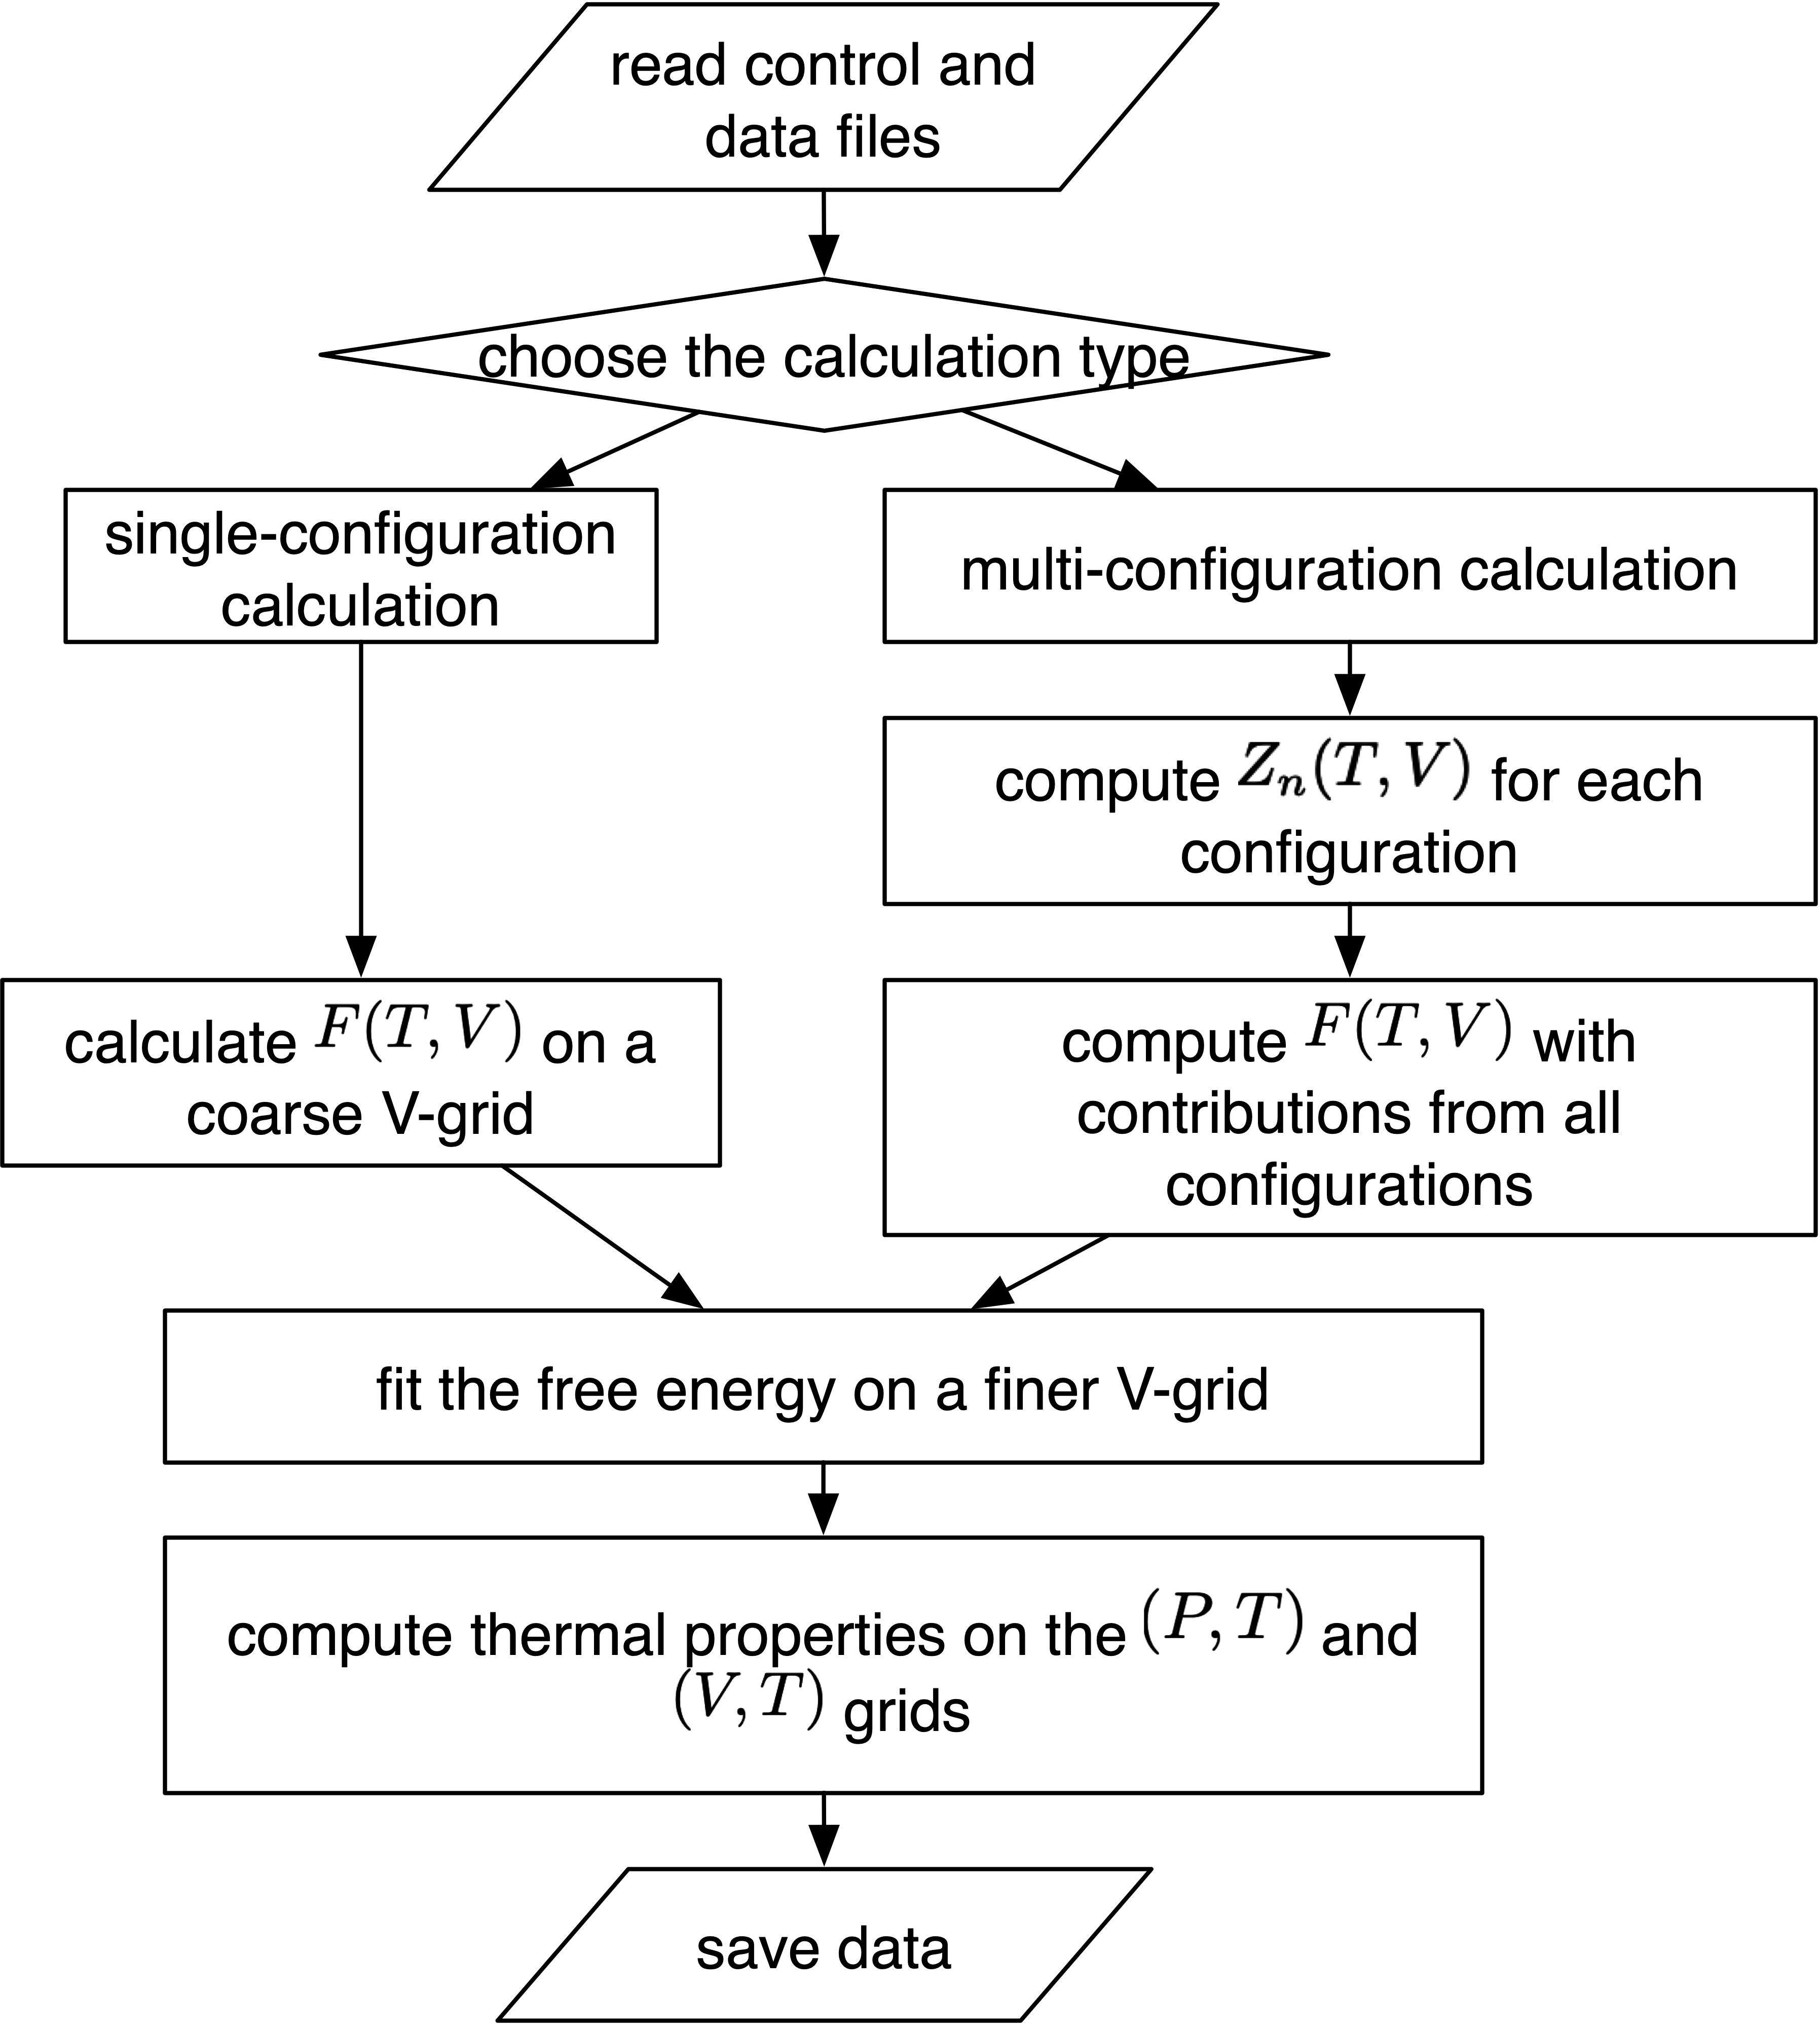
\includegraphics[height=0.95\textheight]{images/flow}%
\end{frame}

\section{Examples}

\subsection{ice VII(disorder)-VIII(order) phase transition}
\begin{frame}{\subsecname}
	\centering
	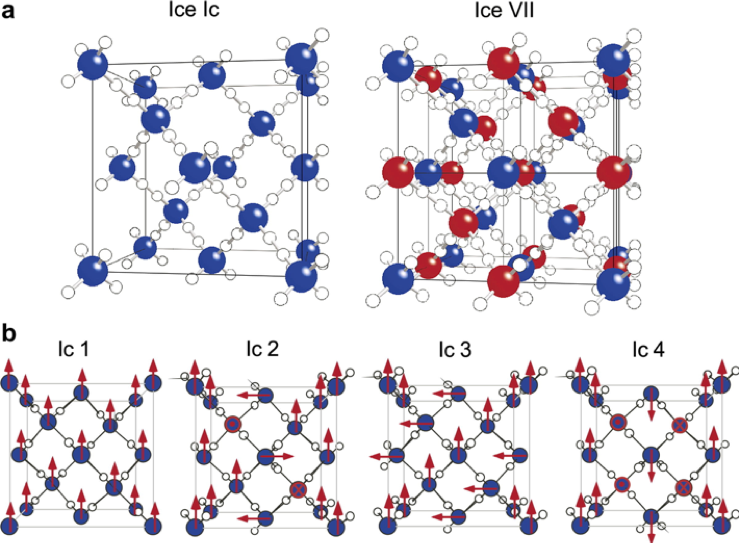
\includegraphics[height=0.9\textheight]{images/ice7}%
\end{frame}

\begin{frame}{\subsecname}
	\begin{figure}
		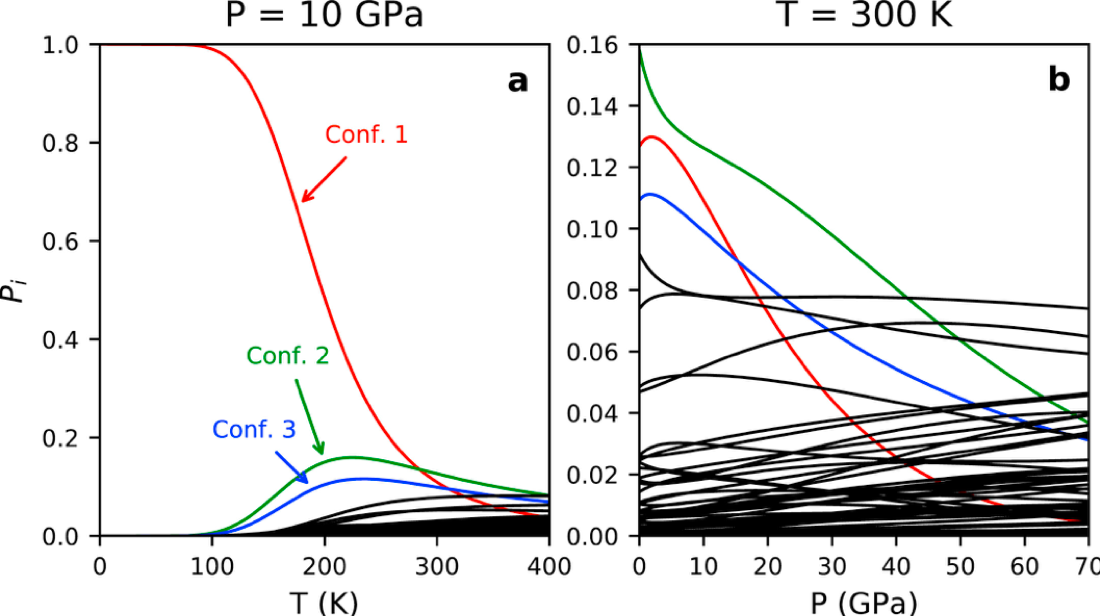
\includegraphics[height=0.75\textheight]{images/ice_prob}%
		\caption{Possibilities $P_i(V, T) = \frac{g_i \exp\Big(\frac{-E_i(V)}{k_B T}\Big)}{Z(V, T)}$ of the $52$ configurations}
	\end{figure}
\end{frame}

\begin{frame}{\subsecname}
	\begin{columns}
		\begin{column}{0.45\textwidth}
			\begin{figure}
				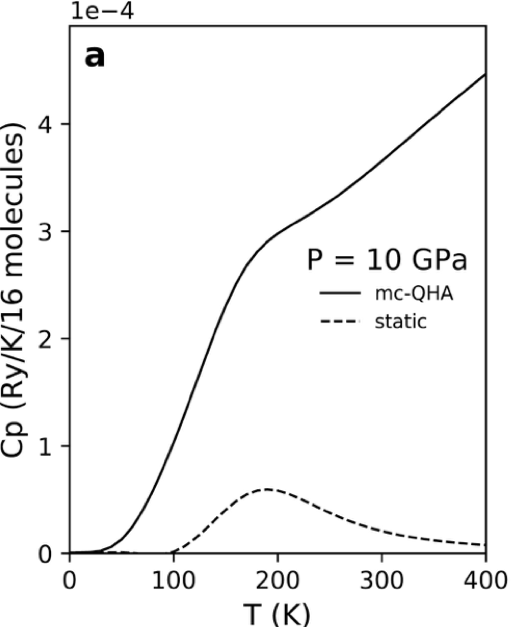
\includegraphics[width=\columnwidth]{images/cp}%
			\end{figure}
		\end{column}

		\begin{column}{0.45\textwidth}
			\begin{figure}
				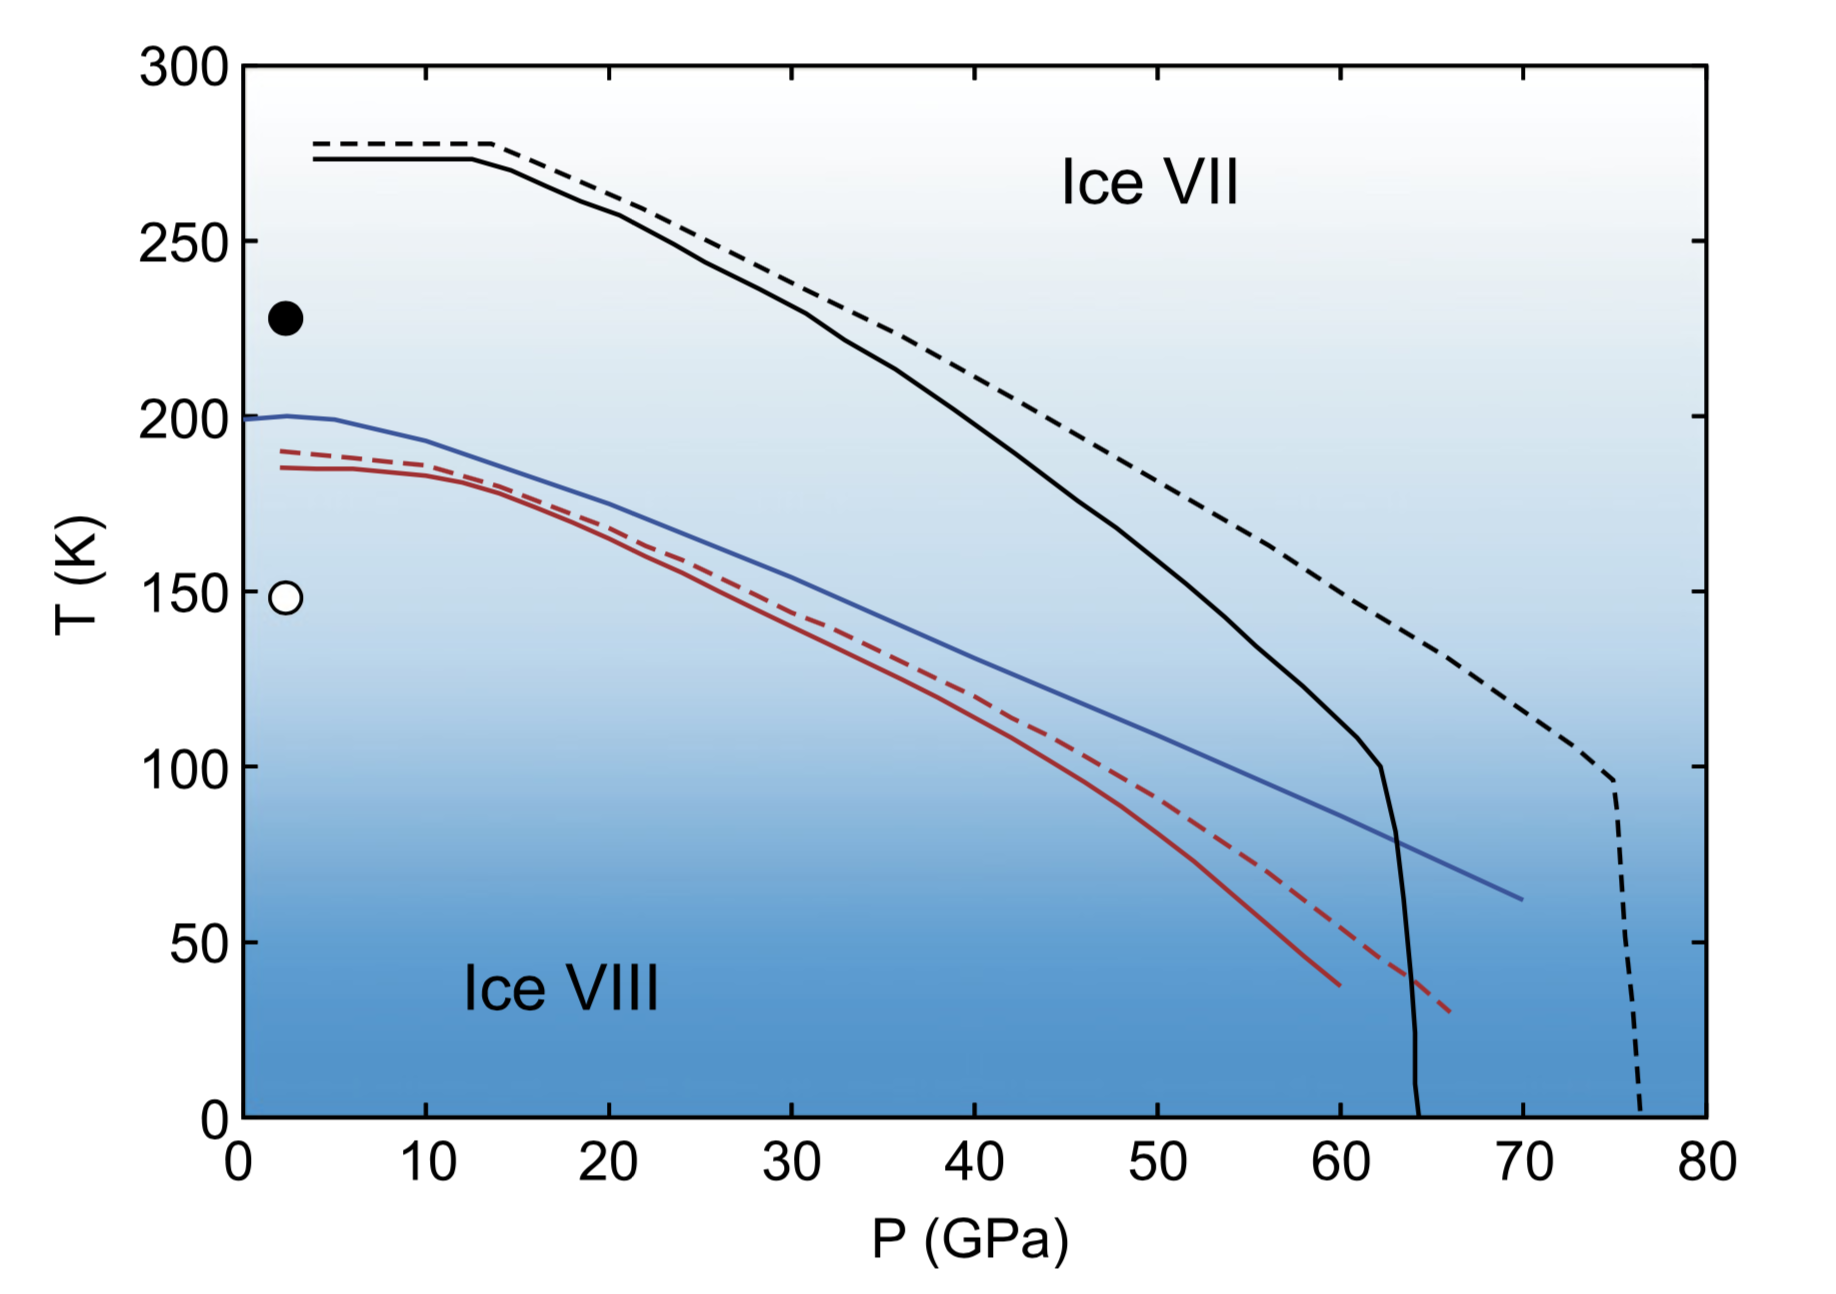
\includegraphics[width=\columnwidth]{images/boundary}%
			\end{figure}
		\end{column}
	\end{columns}
\end{frame}

\subsection{stability of hydrous defects in \ce{Mg2SiO4}-forsterite}
\begin{frame}[allowframebreaks]{\subsecname}
	\begin{columns}
		\begin{column}{0.4\textwidth}
			\begin{figure}
				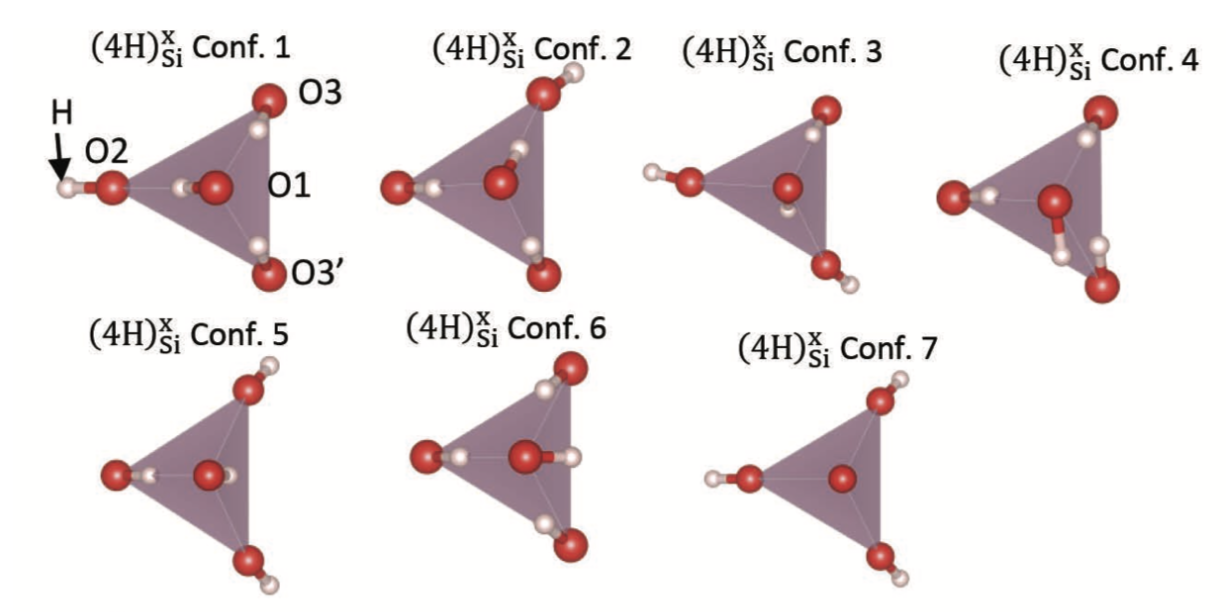
\includegraphics[width=\columnwidth]{images/si}%
				\caption{Configurations of \ce{(4H)^X_{Si}}
				defects. Pink polyhedra represent vacant \ce{Si} sites.}
			\end{figure}
		\end{column}

		\begin{column}{0.4\textwidth}
			\begin{figure}
				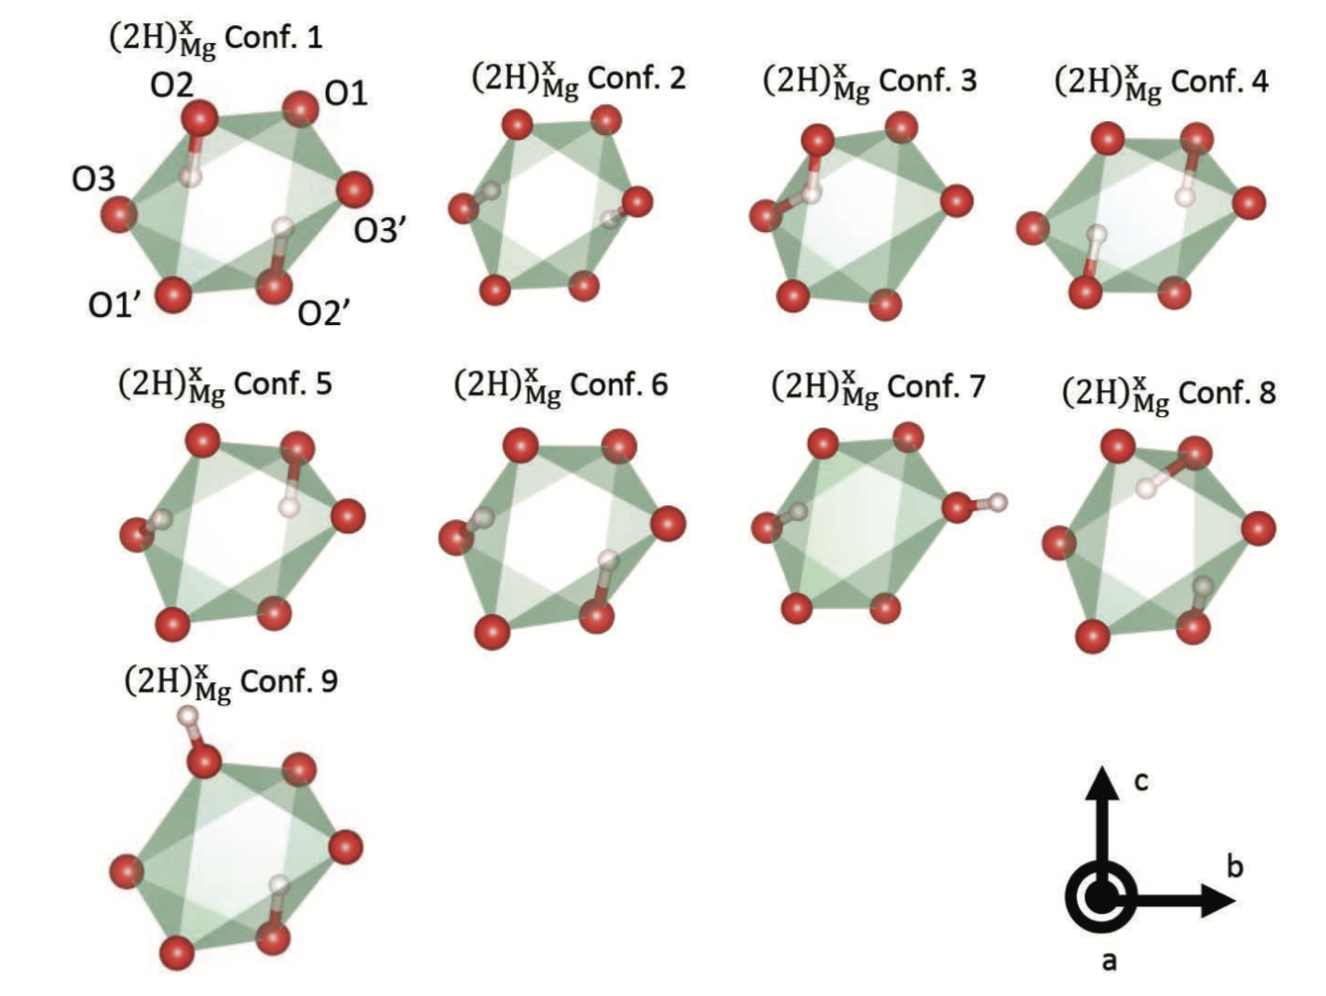
\includegraphics[width=\columnwidth]{images/mg}%
				\caption{Configurations of \ce{(2H)^X_{Mg}}
				defects. Green polyhedra represent vacant \ce{Mg} sites.}
			\end{figure}
		\end{column}
	\end{columns}

	\begin{figure}
		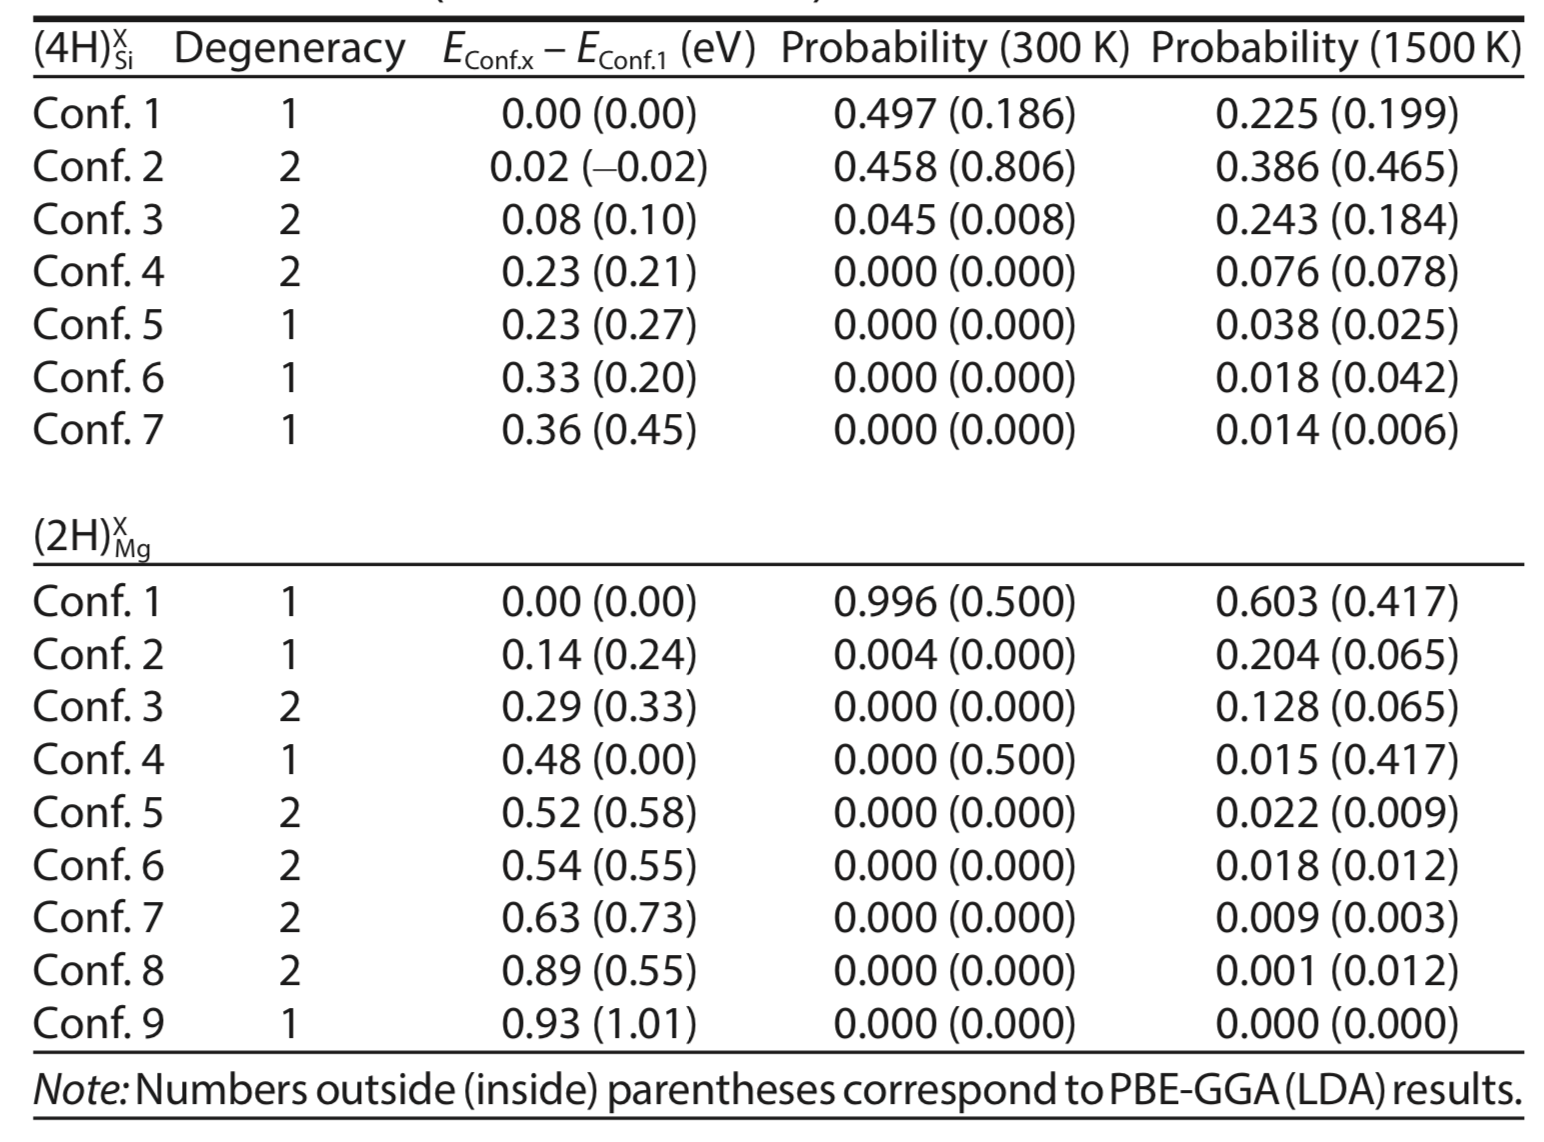
\includegraphics[height=0.8\textheight]{images/simg}%
		\caption{Degeneracies, relative energies, and probabilities of various defects (static calculation)}
	\end{figure}
\end{frame}

\section{Conclusion}

\subsection{Comparisons with other codes}
\begin{frame}{\subsecname}
	\begin{columns}
		\begin{column}{0.45\textwidth}
			\texttt{qha}\\
			\begin{itemize}[<+(1)->]
				\item addresses multi-configuration systems
				\item $G(T,p) = F(T, V) - \Big( \frac{ \partial F }{ \partial V } \Big)_T V$
				\item directly sample the free energy in Brillouin zone
				\item uses JIT techniques to speedup computation
			\end{itemize}
		\end{column}

		\begin{column}{0.45\textwidth}
			other codes\\
			\begin{itemize}
				\item address the thermodynamic properties of single configuration systems
				\item $G(T,p)= \min_{V}[F(T,V)+pV]$ \footnotemark
				\item integrate the vibrational density of states $g(\omega)$ to get $F$ \footnotemark
			\end{itemize}
		\end{column}
	\end{columns}
	\setcounter{footnote}{5}
	\footcitetext{phonopy}
	\stepcounter{footnote}
	\footcitetext{Petretto:2018gg}
\end{frame}

\subsection{Applications and extensibility}
\begin{frame}{\subsecname}
	\begin{columns}
		\begin{column}{0.45\textwidth}
			\begin{figure}
				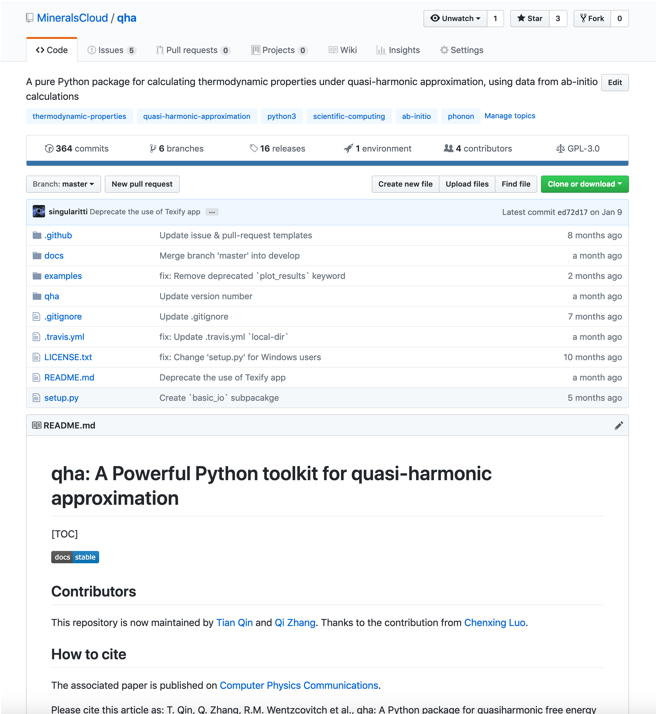
\includegraphics[height=0.7\textheight]{images/website}%
				\captionsetup{labelformat=empty}
				\caption{\scriptsize\url{https://github.com/MineralsCloud/qha}}
			\end{figure}
		\end{column}

		\begin{column}{0.45\textwidth}
			\begin{itemize}[<+(1)->]
				\item Applications to materials research
				      \begin{itemize}
					      \item investigate thermoelastic properties of materials \footnotemark
					      \item investigate metals with its phonon frequencies varying at different temperature
				      \end{itemize}
				\item Applications to geophysical research
				      \begin{itemize}
					      \item calculate the geotherm and isentrope \footnotemark
					      \item calculate the isotope ratio and isotope fractionation factor
				      \end{itemize}
			\end{itemize}
		\end{column}
	\end{columns}
	\setcounter{footnote}{7}
	\footcitetext{Wu:2011ea}
	\stepcounter{footnote}
	\footcitetext{Cardona:2017dd}
\end{frame}

\begin{frame}{\secname}
	\begin{itemize}[<+(1)->]
		\setlength\itemsep{1em}
		\item Implement a fast, easy-to-use, Python package \texttt{qha} for tranditional QHA calculations
		\item \texttt{qha} can calculate multi-configuration system's equation of state and the thermodynamic properties
	\end{itemize}
\end{frame}

\section{Acknowledge\-ments}
\begin{frame}{\secname}
	\begin{itemize}
		\item NSF EAR-1503084, NSF EAR-1341862, NSF EAR-1348066
		\item Stampede2 at the Texas Advanced Computing Center (TACC), University of Texas at Austin
	\end{itemize}
\end{frame}

\section{References}
\begin{frame}[allowframebreaks]{\secname}
	\printbibliography
\end{frame}

\end{document}